\documentclass[13pt]{article}

\title{Relazione 6: Esplorazione Numerica della Mappa Logistica}
\author{Antonio Michele Miti}

\usepackage{amsmath}
\usepackage{amsfonts}
\usepackage[utf8]{inputenc}
\usepackage[italian]{babel}
\usepackage{listings}
\usepackage{textcomp}
\usepackage{graphicx}
\usepackage{subfigure}
\usepackage{rotating}
\usepackage{caption}
\usepackage{latexsym}
\usepackage{epstopdf}
\usepackage{eepic,epic,eepicemu}
\usepackage{color}
\pagestyle{headings}
\definecolor{listinggray}{gray}{0.9}
\definecolor{lbcolor}{rgb}{0.95,0.95,0.95}
\lstset{
	backgroundcolor=\color{lbcolor},
	rulecolor=,
	language=C++,
        basicstyle=\scriptsize,
        upquote=true,
        aboveskip={1.5\baselineskip},
        columns=fixed,
        showstringspaces=false,
        extendedchars=true,
        breaklines=true,
        prebreak = \raisebox{0ex}[0ex][0ex]{\ensuremath{\hookleftarrow}},
        frame=single,
        showtabs=false,
        showspaces=false,
        showstringspaces=false,
        identifierstyle=\ttfamily,
        keywordstyle=\color[rgb]{0,0,1},
        commentstyle=\color[rgb]{0.133,0.545,0.133},
        stringstyle=\color[rgb]{0.627,0.126,0.941},
}
\addtolength{\hoffset}{-1.25cm}
\addtolength{\voffset}{-1.80cm}
\addtolength{\textwidth}{1cm}
\addtolength{\textheight}{3.80cm}
\newtheorem{legge}{Definizione}

\begin{document}
\maketitle
\begin{abstract}
Lo scopo di questo articolo è di mostrare graficamente, attraverso una costruzione numerica, le proprietà fondamentali della mappa logistica: punti periodici, autosimilarità del grafico (struttura frattale) e pseudocaoticità in determinati valori.

Inoltre, attraverso l'esplorazione grafica, si cerca di dare una stima qualitativa della \emph{costante di Feigenbaum}, rapporto limite tra biforcazioni successive.

	
\end{abstract}

%\tableofcontents

\section{Introduzione}

Quando si considera una generica \emph{mappe reale in dimensione 1} (funzione continua $ f: \mathbb{R} \supseteq I \rightarrow I$) si è interessati a studiare alcuni punti peculiari: i punti fissi e punti periodici, loro diretta generalizzazione.

	\begin{legge}[Punto Fisso]
	$x_{F} \in I$ è punto fisso della mappa $f(x)$ quando:	
		\begin{equation}
		f(x_{F}) = x_{F}
		\end{equation}
	\end{legge}

	\begin{legge}[Punto Periodico di periodo $N$]
	Sia $f^{n}$ la mappa costruita componenendo N volte la mappa $f(x)$ con se stessa (è perciò detta iterata N-sima). 

$x_{0} \in I$ è punto periodico di periodo N della mappa quando:	
		\begin{equation}
		f^{n}(x_{0}) = x_{0}
		\end{equation}
ovvero $x_{0}$ è punto fisso della mappa iterata N-sima. 
	\end{legge}

La trattazione di questi oggetti è particolarmente utile in sistemi dinamici, gli operatori di evoluzione temporale sono appunto mappe continue sullo spazio delle fasi, in virtù di questo la successione di punti $\{x_{0}, x_{1}, x_{2}, \ldots\} \subset I $ costruita interando in modo discreto la mappa $f(x)$, è detta \emph{orbita}.

\subsection{Stabilità dei punti Fissi}

L'importanza dei punti fissi è quindi chiara, la continua applicazione della mappa a tali punti restituisce sempre come immagine il punto stesso. Diviene quindi naturale chiedersi se questi punti costituisco un "attrattore", ovvero se il punto fisso sia di accumulazione per la generica orbita costruita a partire da un punto "vicino" ad esso.

Si consideri una mappa sufficientemente regolare $ f(x_{n}) = x_{n+1}$ con $x_{F}$ punto fisso.

La regolarità permette di sviluppare in serie di Taylor la mappa attorno al punto $x_{F}$:

	\begin{equation}
		x_{1} = f(x_{F} + \varepsilon) =  \sum_{i = 0}^{\infty} f^{(n)}(x_{F}) \dfrac{\varepsilon^{n}}{n!}
	\end{equation}

se $x_{0}$ è molto vicino a $x_{F}$ si avrà $\mid \varepsilon_{0} \mid \ll 1$ per cui è possibile rappresentare la mappa con lo sviluppo troncato al primo ordine :

	\begin{equation}
		x_{1} = x_{F} + f'(x_{F})\varepsilon_{0}
	\end{equation}

per il punto successivo dell'orbità si ottiene in modo simile:

	\begin{equation}
		x_{2} =f(x_{F} + f'(x_{F})\varepsilon_{0}) = x_{F} f'(x_{F}\varepsilon_{1})
	\end{equation}

dove $\varepsilon_{1} = f'(x_{F})\varepsilon_{0}$ quindi è ancora abbastanza piccola da rendere approssimabile la mappa con lo sviluppo troncato, e così via per tutti i punti successivi.
Ne risulta l'orbita ${x_{0}, x_{1}, x_{2}, \ldots}$.

Ora non resta che stabilire se la successione converga ad $x_{f}$ o meno.
Per farlo è sufficiente studiare la convergenza della successione delle distanze: $$\{x_{0} - x_{F}, x_{1} - x_{F}, x_{2} - x_{F}, \ldots\} \, = \, \{\varepsilon_{n}\} $$

Per la costruzione precedente è evidente che il termine n-simo valga:

	\begin{equation}
		\varepsilon_{n+1} =f'(x_{F})\varepsilon_{n}) \longrightarrow \varepsilon_{n} = [ f'(x_{F}) ]^{n} \varepsilon_{0}
	\end{equation}

quindi la convergenza dell'orbita è determinata dalla convergenza del limite $$ \lim_{n\rightarrow\infty}[ f'(x_{F}) ]^{n} = K.$$

In conclusione:
	\begin{itemize}
	\item[-] se $\vert f'(x_{F}) \vert < 1$ allora $K=0$, quindi $x_{f}$ è detto \emph{Attrattore}.
	\item[-] se $\vert f'(x_{F}) \vert > 1$ allora $K=\infty$, quindi $x_{f}$ è detto \emph{Repulsore}.
	\end{itemize}
il caso limite $\vert f'(x_{F}) \vert = 1$ rimane indeterminato.


\subsection{Biforcazioni}
Si consideri ora una mappa $f_{\lambda}(x_{n})$ dipendente in modo continuo da un parametro $\lambda$, la mappa potrà ammettere uno o più punti fissi (o periodici) la cui posizione dipenderà in generale da un parametro.

Siccome la mappa dipende in modo regolare da $\lambda$ si può indentificare una curva parametrizzata $x_{0}(\lambda)$ che descrive la posizione di questo punto fisso al variare del parametro.

Per quanto detto prima la stabilità di un punto fisso dipende dalla derivata $f'_{\lambda}(x) $ quindi al variare del parametro varia anch'essa, e il punto fisso può passare da attrattore a repulsore e viceversa oppure possono nascere dei nuovi punti periodici.

I valori critici di $\lambda$ per cui avvengono tali modificazioni si definiscono \emph{biforcazioni}.

Se la mappa è almeno regolare di classe $C^{1}$ si ha che $f'_{\lambda}(x) $ varia in modo continuo al variare del parametro, quindi i fenomeni di biforcazione possono avvenire solo nel momento in cui il punto critico $x_{0}(\lambda)$ cambia di regolarità, ovvero quando $f'_{\lambda}(x_{0}(\lambda)) = \pm 1$ .


 
\section{Caso di Studio}

\paragraph{La Mappa Logistica}
E' la funzione regolare:
	\begin{equation}
		x_{n+1} = f_{r}(x_{n}) = r \, x_{n}(1-x_{n})
	\end{equation}
dipendente con continuità dal parametro $r$.

Si nota che questa funzione rappresenta una mappa sul intervallo $I=[0,1] \subset \mathbb{R}$ solo per determinati valori di r. Infatti calcolando che il massimo:
	\begin{displaymath}
		\dfrac{\textrm{d}x_{n+1}}{\textrm{d} x_{n}} = r(1-2x_{n})=0 \rightarrow x_{n \, \textrm{max}} = \dfrac{1}{2}
	\end{displaymath}
si trova che:
	\begin{displaymath}
		f(x_{n \, \textrm{max}}) = \dfrac{r}{4} \qquad \in I \Leftrightarrow 0\leq r \leq 4
	\end{displaymath}


Da un calcolo elementare è evidente che la mappa presenta sempre 2 punti fissi $0$ e $\frac{r-1}{r}$ la cui stabilità varia al variare del parametro.

Calcolando la derivata della mappa $f'_{r}(x) = r \, (1-2x) $ nei punti fissi si ottiene:
	\begin{equation}
		f'_{r}(0) = 0 \qquad f'_{r}(\frac{r-1}{r})= 2-r
	\end{equation}
Quindi per $\lambda < 1$ il primo è un attrattore e il secondo un repulsore; per $1 < \lambda < 3$ si invertono di stabilità mentre per $\lambda > 3$ diventano entrambi repulsori.

La biforcazione in $r = 3$ è particolarmente interssante perchè da vita a una biforcazione con raddoppio del periodo, in sostanza nascono 2 nuovi punti periodici di periodo 2 che fungono da attrattori.

La cosa si può mostrare visualizzando le intersezioni dei grafici della funzione iterata 2 volte $f^{2}_{r}(x)$ sul dominio $[0,1]$ con la retta $y=x$, che di fatto sono i punti fissi della mappa, con parametro r fissato un po' prima di 3 e un po' dopo \ref{fig:quadrobif}.

\begin{figure}[!h]
\centering
\includegraphics[width=13cm,keepaspectratio]{picture/quadrodispense}
\caption{La biforcazione con raddoppio del periodo per la mappa logistica in corrispondenza a $r =3$. Si nota subito che dopo $r =3$ l'iterata seconda della mappa presenta 2 nuovi intersezioni.}
\label{fig:quadrobif}
\end{figure}

Quando una mappa possiede due attrattori di periodo 2 accade che, partendo da un punto $x_{0}$ casuale, tutte le iterate pari $f^{2j}_{r}(x_{0})$ convergono ad un attrattore, mentre tutte le iterate dispari $f^{2j+1}_{r}(x_{0})$ convergono all'altro.

La spiegazione è evidente: per la definizione di attrattore l'immagine $f^{2}$ su un intorno del primo punto periodico è ancora un intorno del punto ma di dimensione minore. Considerando quindi l'immagine di $f$ su questo intorno per la continuità di f è ancora un intorno che al aumentare delle iterazioni di $f^{2}$ tenderà esattamente al secondo attrattore. 

Diventa spontaneo chiedersi se anche la mappa $f^{2}_{r}(x)$ presenta una biforcazionecon raddopio del periodo al cresere di r, oppure, in altre parole, presenti 4 punti di periodo 4.

Proseguire l'indagine con calcoli algebrici diventa piuttosto lungo, conviene quindi ricorrere all'esplorazione numerica.




\section{Metodologia}

Con il termine di "esplorazione numerica" non si intende nient'altro che rappresentare l'immagine della mappa logistica $f^{n}_{r}(x_{0})$ variando uno dei parametri e fissando tutti gli altri.

La Mappa Logistica  presenta solo 3 possibili parametri da manipolare $(r, \, x_{0}, \, N)$ , ne risulta un implementazione \emph{C++} molto semplice:

\begin{lstlisting}[frame=single]
double mappalogistica( double r, double x0, int N)
	{
	for(int i=0;i<=N; i++)x0=r*(x0-x0*x0);
	return(x0);
	}
\end{lstlisting}
.

\subsection{Comportamento generale}
%mappa2 zoom sulle biforcazioni,

L'operazione più spontanea per avere una visualizzazione grafica della mappa consiste nel mettere in grafico le posizioni dei punti di accumulazione delle orbite attrattive in funzione del parametro $r$.

L'unico modo per ottenere gli attrattori consiste nel partire da un punto iniziale $x_{0}$ scelto in modo casuale (con la funzione random di \emph{C++}) tra 0 e 1, calcolare un transiente di un certo numero N di punti, ovvero iterare la mappa senza riportare i punti sul grafico in modo che l'orbita si avvicini sufficientemente all'attrattore, e successivamente stampare alcuni dei punti successivi ( visto che si tratta di biforcazioni è opportuno stamparne $2^{k}$).

La figura ottenuta dovrebbe rendere evidente la presenza di biforcazioni con raddoppiamento del periodo succesive alla prima, graficamente questo fenomeno si manifesta appunto con un raddoppiamento dei punti di accumulazione rappresentati sul grafico.

Chiaramente ogni metodo computazionale rappresenta l'andamento su valori discreti di $r$ (si tratta pur sempre di campionamenti), siccome il grafico va incontro a continue biforcazioni la densità di punti utilizzati per rappresentare ogni ramo verrà dimezzata di volta in volta

Qualora si volesse visualizzare un ingrandimento della figura è preferibile ricalcore i punti, facendo variare $r$ sull'intervallo opportuno e se si è in presenza di numerose biforcazioni, stampare molti più punti per lo stesso valore del parametro.

\subsection{Punti di Biforcazione, costante di Feigenbaum}

La tesi sostenuta da M. Feigenbaum a proposito di questa mappa è che il rapporto della distanze tra 2 biforcazioni consecutive e le 2 successive tende ad una costante al tendere all'infinito delle biforcazioni.

Formalmente: siano $r_{j}$ i valori critici tali per cui l'orbita di periodo $2^{j-1}$ biforca in un'orbita di periodo $2^{j}$, allora :
\begin{equation}
		\lim_{j\to \infty}\dfrac{r_{j}-r_{j-1}}{r_{j+1}-r_{j}} =  4.6692\ldots \qquad .
	\end{equation}

Per dimostrare questa asserzione è necessario individuare il parametro $r$ relativo ad un certo numero di biforcazioni, un calcolo rapido può svolgersi semplicemente ricordandosi che la prima biforcazione (calcolata in modo algebrico) si trova per $r_{1} = 3$ e valutando alcuni dei $\lambda_{j}$ semplicemente individuandone l'ascissa dalle figure costruite con il procedimento visto nel punto precedente.

Questo metodo è molto impreciso per diversi motivi: il problema principale è dato dalla velocità di convergenza all'attrattore per punti vicini alla biforcazione è molto lenta, quindi sono richieste molte iterazioni per fissare in modo chiaro il punto, il secondo problema è fissato dal tempo di esecuzione del calcolatore: leggere un numero su un grafico richiede una buona definizione dei punti che a sua volta richiede un grande numero di operazioni quindi un tempo di calcolo molto grande.

\subsection{Convergenza all' attrattore}

Dimostrare che per valori di $r$ che presentano biforcazioni, la mappa salta da un intorno del punto periodico all'altro è graficamente molto semplice, è sufficiente stampare le prime iterazioni della mappa a partire da un valore $x_{0}$ scelto casualmente, mettendo in ascissa il numero del iterata e in ordinata il valore in uscita.

Dallo stesso grafico si può dare anche una rappresantazione qualitativa della velocità di convergenza della $f^{n}_{r}(x_{0})$ all'aumentare di n, per valori di $r$ critici prossimi al punto di biforcazione della mappa.
%in generale (mappa3) e sui punti di biforcazione (mappa 4)

Siccome si è interessati a localizzare i punti di biforcazione può essere utile visualizzare come varia la geometria della biforcazione all'aumentare del numero di iterazioni utilizzate per calcolare il transiente iniziale. 

Per farlo è sufficiente generare un certo numero di grafici che rappresentano l'intorno della prima biforcazione come spiegato nel punto $3.1$,  con un diverso numero di iterazioni del transiente iniziale.

\subsection{Insorgenza del Caos}

Un possibile modo per visualizzare l'insorgenza del caos è costruire un grafico in modo simile al punto 3.1, con la differenze di stampare per ogni $r$ solo l'n-simo valore relativo e di usare come valore iniziale sempre lo stesso numero.

In questo modo si ha che per quei valori di $r$ in cui la mappa presenta un numero finito di rami, il grafico presenti solo uno di essi.

Nel momento in cui il parametro entra nella regione caotica, dove gli attrattori e il loro periodo tendono all'infinito non sarà più visibile il ramo ben definito ma apparirrano punti distribuiti in modo apparentemente casuale in un sottointervallo del dominio.

\section{Risultati}

I grafici \ref{fig:general} e \ref{fig:general_zoom} presentano la struttura della mappa. La figura presenta evidentemente degli aspetti sorprendenti.

Al crescere di $r$ si osservano chiaramente le biforcazioni che generano le orbite di periodo 2,4,8,e così via.
Come previsto i raddoppi del periodo si succedono a cascata fino a che la figura non si fa confusa e si ha la sensazione che da un punto in poi l'orbita riempa un intero intero intervallo, con il continuo raddoppiamento del periodo la dinamica tende a diventare caotica.

Si osservano in seguito anche delle bande bianche quasi vuote, ingrandendo il grafico in quelle aree ( figura \ref{fig:isole}) si scopre che la mappa si regolarizza di nuovo, si ritrova nel piccolo di nuovo la figura iniziale della mappa .

\paragraph{\textbf{b}iforcazioni}.

Dallo studio del grafico \ref{fig:bifo} si ottengono i seguenti valori del parametro $r$ relativo alle biforcazioni:
\begin{displaymath}
\centering
\begin{array}{|c|c|c|}
\hline
\textrm{Biforcazione} & \textrm{r} & \textrm{stima costante Feigenbaum} \\
\hline
\hline
I	 & 	3,000000000	 & 	\\
\hline
II	 & 	3,449489743	 & 	4,75159 \\
\hline
III	 & 	3,544087500	 & 	4,65529 \\
\hline
IV	 & 	3,564408000	 & 	4,67138 \\
\hline
V	 & 	3,568758000	 & 	4,65938 \\
\hline
VI	 & 	3,569691600	 & 	4,67571 \\
\hline
VII	 & 	3,569891270	 & 	4,67146 \\
\hline
VIII	 & 	3,569934013	 & 	4,66239 \\
\hline
\end{array}
\end{displaymath}

il numero dei punti non è sufficiente per stimare il valore limite della costante di Feigenbaum ma presenta comunque un buon accordo con i valori teorici, considerando un errore sulla stima della biforcazione di almeno $\pm 1\%$.

Nella figura 5 si evidenzia l'andamento del orbita per mappe con valore r relativo alle prime biforcazioni, come predetto la successione passa dall'intorno di un punto periodico all'altro convergendo rapidamente all'attrattore.


%generali
\begin{sidewaysfigure}[!h]
\includegraphics[width=24cm,keepaspectratio]{picture/mappa7/mappabif-joined}
\caption{Comportamento generale della mappa su tutto il dominio.}
\label{fig:general}
\end{sidewaysfigure}

\begin{sidewaysfigure}[!h]
\includegraphics[width=24cm,keepaspectratio]{picture/mappa7/mappabiforcazioni1-joined}
\caption{Comportamento generale della mappa, ingrandimento sulla zona critica del dominio.}
\label{fig:general_zoom}
\end{sidewaysfigure}

%biforcazioni
\begin{sidewaysfigure}[!h]
\includegraphics[width=24cm,keepaspectratio]{picture/quadro_1}
\caption{Individuazione Delle prime biforcazioni della mappa Logistica.}
\label{fig:bifo}
\end{sidewaysfigure}





%
%convergenza agli attrattori
\begin{figure}[!htbp]
	\caption{Rappresentazione grafica delle prime iterate della mappa logistica negli intervalli tra la prima, la seconda e la terza biforcazione.}

	\subfigure{\includegraphics[width=11cm,height=7cm]{picture/mappa3/2punti}}\\
 	\subfigure   {\includegraphics[width=11cm,height=7cm]{picture/mappa3/4punti}}\\
 	\subfigure   {\includegraphics[width=11cm,height=7cm]{picture/mappa3/8punti}}\\
	
\end{figure}





\clearpage
\paragraph{Convergenza nell'intorno della biforcazione}

Nell'intorno dei punti critici, dove la figura \ref{fig:bifo} presenta una biforcazione, le orbite convergono all'attrattore molto debolmente come visibile nel grafico \ref{fig:quadrobif}.

Questo fa si che la convergenza all'attrattore richieda un transiente molto lungo, l'effetto di un transiente non sufficiente si manifesta nella figura come uno sdoppiamento.

Si ha l'impressione che la biforcazione avvenga prima ma guardando meglio si nota che molti punti cadono distribuiti tra i 2 rami. Questo effetto è mostrato nella figura \ref{fig:confrontn}.
\begin{figure}[!h]
\centering
\includegraphics[width=10cm,keepaspectratio]{picture/mappa3/r=3}
\caption{Orbita della mappa sulla prima biforcazione, quindi con r=3.}
\label{fig:quadrobif}
\end{figure}
%
%convergenza della biforcazione
\begin{figure}[!h]
\centering
\includegraphics[width=10cm,keepaspectratio]{picture/mappa5/confronto_n}
\caption{Confronto tra il grafico della prima biforcazione (r = 3 ) ottenuto con diversi transienti iniziali. In sostanza viene visualizzata la convergenza della mappa all'attrattore nella prossimità di r=3.}
\label{fig:confrontn}
\end{figure}

\paragraph{Struttura Frattale della mappa}

Un frattale è un oggetto geometrico che si ripete nella sua struttura allo stesso modo su scale diverse. Questa caratteristica è spesso chiamata auto-similarità (self-similarity).

Alla base dell’auto-similarità sta una particolare trasformazione geometrica chiamata omotetia: trasformazione geometrica del piano o dello spazio, che dilata o contrae gli oggetti, mantenendo invariati gli angoli ossia la forma (nel senso intuitivo del termine).

Un frattale è un ente geometrico che mantiene la stessa forma se ingrandito con una omotetia opportuna, detta omotetia interna.

La figura \ref{fig:bifo} ha evidenti proprietà di auto-similarità, ad esempio nella figura \ref{fig:frattali}  ingrandendo settori sempre più piccoli della figura si ottiene praticamente la medisima immagine.

Questo fenomeno però non è un esclusiva della zona non caotica, anche dopo il valore critico la mappa presenta delle isole di stabilità che ripropongo uno schema identico a quello visto precedentemente come è visibile nella figura \ref{fig:isole}. Nella stessa figura si nota inoltre che l'isola di stabilità presenta anche lei a sua volta una zona caotica che contiene  delle bande di stabilità. Si potrebbe continuare almeno fin che la precisione non renda impossibile il calcolo numerico.
%
%frattalità
\begin{sidewaysfigure}[!h]
\includegraphics[width=22cm,keepaspectratio]{quadro_1}
\caption{Struttura frattale della mappa logistica. Stampa di alcuni ingrandimenti della mappa nei pressi delle  prime 4 biforcazioni. E' evidente l'auto-similarità della figura.}
\label{fig:frattali}
\end{sidewaysfigure}


%isole di regolarità nel caos
\begin{sidewaysfigure}[!h]
\centering
\includegraphics[width=24cm,keepaspectratio]{picture/mappa4/quadro_1}
\caption{Ingrandimento progressivo di un isola di stabilità nella zona caotica della mappa.}
\label{fig:isole}
\end{sidewaysfigure}




\clearpage
\paragraph{Caoticità della Mappa}

Costruendo il grafico \ref{fig:identicaos} come descritto nel paragrafo 3.4 si dimostra che la mappa entra in una regione caotica per valori $r > \sim 3,57 $.

Dai grafici precedenti inoltre si vede inoltre che le orbite assumono valori compresi su tutto l'intervallo $ I=[0,1]$ solo per $r = 4$.


\begin{figure}[!h]
\centering
\includegraphics[width=14cm,keepaspectratio]{picture/mappa7/zoomcaos}
\caption{Metodo di inviduazione della regione caotica. La regione caotica incomincia approssimativamente quando r supera $3,57$.}
\label{fig:identicaos}
\end{figure}

A questo punto è possibile chiedersi se queste figure apparentemente casuali possano essere utilizzate come generatore pseudo random.
Per stabilire l'effettiva casualità della regione caotica non c'è un criterio, ci si può limitare a stabilire se la distribuzione dei punti di un orbita qualsiasi della mappa con r=4 è regolare o no.

\begin{figure}[!h]
\centering
\includegraphics[width=10cm,keepaspectratio]{picture/mappacaos/istocaos}
\caption{Istogramma dei primi 50000 punti del orbita per la mappa r=4.}
\label{fig:istocaos}
\end{figure}


\begin{figure}[!h]
\centering
\includegraphics[width=10cm,keepaspectratio]{picture/mappacaos/istocaoszoom}
\caption{Ingrandimento del grafico \ref{fig:istocaos} nella parte centrale}
\label{fig:zoomistocaos}
\end{figure}

Dalla figura \ref{fig:istocaos} risulta evidente che la distribuzione non è regolare su tutto l'intervallo, i valori vicino ai bordi dell'intervallo sono maggiormente probabili, quindi la mappa così com'è non rappresenta un buon generatore di numeri casuali tra 0 e 1.
Però dalla figura \ref{fig:zoomistocaos}, ingrandimento dell'istogramma precedente nel punto medio dell'intervallo $[0,1]$ si nota che l'istogramma si regolarizza, la distribuzione sembra pressochè uniforme in questo sottointervallo.

L'intuizione precedente porta a chiedersi come appare la distribuzione di probabilità dell'orbita di cui prima si è costruito l'istogramma.
Tale grafico può essere ottenuta in modo analogo all'istogramma rendendo molto piccole (in modo da approssimare l'intervallo infinitesimo)le basi delle colonne dell'istogramma.
In questo modo si ottiene la figura \ref{fig:densit}, come visto prima la funzione densità di probabilità per i valori dell'orbita sembra tendere alla distribuzione costante per l'aperto $(0,1)$.
\begin{figure}[!h]
\centering
\includegraphics[width=10cm,keepaspectratio]{picture/mappacaos/superisto}
\caption{Funzione densità di probabilità per i risultati della mappa logistica con r = 4. E' costruito aumentanto molto la suddivisione in intervalli dell'istogramma.}
\label{fig:densit}
\end{figure}





\clearpage
\begin{thebibliography}{99}
\bibitem{recipe}\emph{Numerical recipes in C++}
\bibitem{knuth}Knuth D. \emph{The Art of Computer Programming}
\bibitem{hilde}Hildebrand F. \emph{Introduction to Numerical Analysis}, 2nd.ed.
\end{thebibliography}
\end{document}
